\documentclass[a4paper,20pt]{article}
\usepackage{amsmath,amssymb,epsf,epsfig,times}
\usepackage{multicol}
\usepackage[all]{xy}
\usepackage{color}
\usepackage{ctex}
\usepackage{subfigure}
\usepackage{url,cite}
\usepackage{tikz}
\usepackage[english]{babel}
\usepackage[utf8]{inputenc}

\usepackage{pdfpages}

%\usepackage{caption}
%
%\usepackage[font=small,labelfont=bf,labelsep=none]{caption}
\usepackage[font=default,labelfont=bf,labelsep=period]{caption}

\usepackage{makecell}
\usepackage{booktabs} %引入三线表
\usepackage{diagbox}
\usepackage{multirow}

\usepackage{fancyhdr}
\usepackage{float}
\usepackage{ulem}

\usepackage{listings}
\usepackage{xcolor}

\usepackage{enumerate}
\lstset{
    basicstyle          =   \sffamily,          % 基本代码风格
    keywordstyle        =   \bfseries,          % 关键字风格
    commentstyle        =   \rmfamily\itshape,  % 注释的风格,斜体
    stringstyle         =   \ttfamily,  % 字符串风格
    flexiblecolumns,                % 别问为什么,加上这个
    numbers             =   left,   % 行号的位置在左边
    showspaces          =   false,  % 是否显示空格,显示了有点乱,所以不现实了
    numberstyle         =   \zihao{-5}\ttfamily,    % 行号的样式,小五号,tt等宽字体
    showstringspaces    =   false,
    captionpos          =   t,      % 这段代码的名字所呈现的位置,t指的是top上面
    frame               =   lrtb,   % 显示边框
}
\lstdefinestyle{Python}{
    language        =   Python, % 语言选Python
    basicstyle      =   \zihao{-5}\ttfamily,
    numberstyle     =   \zihao{-5}\ttfamily,
    keywordstyle    =   \color{blue},
    keywordstyle    =   [2] \color{teal},
    stringstyle     =   \color{magenta},
    commentstyle    =   \color{red}\ttfamily,
    breaklines      =   true,   % 自动换行,建议不要写太长的行
    columns         =   fixed,  % 如果不加这一句,字间距就不固定,很丑,必须加
    basewidth       =   0.5em,
}

\newtheorem{theorem}{Theorem}[section]
\newtheorem{lemma}{Lemma}[section]
\def\proof{\noindent{\it Proof: }}
\def\QED{\mbox{\rule[0pt]{1.5ex}{1.5ex}}}
\def\endproof{\hspace*{\fill}~\QED\par\endtrivlist\unskip}
\newcommand{\re}{\mathbb{R}}
\def\sV{\mathcal{V}}
\def\sS{\mathcal{S}}
\def\sQ{\mathcal{Q}}

\newcommand{\mc}{\mbox{: }}

\newcommand{\normsq}[1]{\left\|#1\right\|^2}
\newcommand{\norm}[1]{\left\|#1\right\|}
%\newcommand{\sgn}[1]{\mbox{sgn}(#1)}
\newcommand{\pde}[2]{\frac{\partial #1}{\partial #2}}
\newcommand{\fundef}[3]{#1:#2\to #3}
\newcommand{\abs}[1]{\left|#1\right|}
\newcommand{\mymatrix}[2]{\left(\begin{array}{#1}#2\end{array}\right)}
\newcommand{\defeq}{\stackrel{\triangle}{=}}
\newcommand{\paren}[1]{\left(#1\right)}
%\theoremstyle{plain} \newtheorem{theorem}{Theorem}
%\theoremstyle{plain} \newtheorem{algorithm}{Algorithm}
\newtheorem{axiom}[theorem]{Axiom}
\newtheorem{definition}[theorem]{Definition}
\newtheorem{assumption}[theorem]{Assumption}
\newtheorem{example}[theorem]{Example}
%\theoremstyle{plain}\newtheorem{lemma}{Lemma}
%\newtheorem{proposition}[theorem]{Proposition}
\newtheorem{remark}[theorem]{Remark}
\newtheorem{corollary}[theorem]{Corollary}

\newcommand{\Acal}{\mathcal{A}}
\newcommand{\Bcal}{\mathcal{B}}
\newcommand{\Ccal}{\mathcal{C}}
\newcommand{\Dcal}{\mathcal{D}}
\newcommand{\Ecal}{\mathcal{E}}
\newcommand{\Fcal}{\mathcal{F}}
\newcommand{\Gcal}{\mathcal{G}}
\newcommand{\Hcal}{\mathcal{H}}
\newcommand{\Ical}{\mathcal{I}}
\newcommand{\Jcal}{\mathcal{J}}
\newcommand{\Kcal}{\mathcal{K}}
\newcommand{\Lcal}{\mathcal{L}}
\newcommand{\Mcal}{\mathcal{M}}
\newcommand{\Ncal}{\mathcal{N}}
\newcommand{\Ocal}{\mathcal{O}}
\newcommand{\Pcal}{\mathcal{P}}
\newcommand{\Qcal}{\mathcal{Q}}
\newcommand{\Rcal}{\mathcal{R}}
\newcommand{\Scal}{\mathcal{S}}
\newcommand{\Tcal}{\mathcal{T}}
\newcommand{\Ucal}{\mathcal{U}}
\newcommand{\Vcal}{\mathcal{V}}
\newcommand{\Wcal}{\mathcal{W}}
\newcommand{\Xcal}{\mathcal{X}}
\newcommand{\Ycal}{\mathcal{Y}}
\newcommand{\Zcal}{\mathcal{Z}}


\def\omegavec{\boldsymbol{\omega}}
\newcommand{\alphabf}{\boldsymbol{\alpha}}
\newcommand{\omegabf}{\boldsymbol{\omega}}
\def\omegavec{\boldsymbol{\omega}}
\newcommand{\taubf}{\boldsymbol{\tau}}
\newcommand{\qbf}{\mathbf{q}}
\newcommand{\ybf}{\mathbf{y}}
\newcommand{\pbf}{\mathbf{p}}
\newcommand{\rbf}{\mathbf{r}}
\newcommand{\ebf}{\mathbf{e}}
\newcommand{\onebf}{\mathbf{1}}
\newcommand{\zerobf}{\mathbf{0}}
\newcommand{\abf}{\mathbf{a}}
\newcommand{\ibf}{\mathbf{i}}
\newcommand{\jbf}{\mathbf{j}}
\newcommand{\kbf}{\mathbf{k}}
\newcommand{\vbf}{\mathbf{v}}
\newcommand{\wbf}{\mathbf{\omega}}
\newcommand{\fbf}{\mathbf{f}}
\newcommand{\zbf}{\mathbf{z}}
\newcommand{\xbf}{\mathbf{x}}
\newcommand{\dbf}{\mathbf{d}}
\newcommand{\Rbf}{\mathbf{R}}
\newcommand{\Tbf}{\mathbf{T}}

\newcommand{\Cbf}{\mathbf{C}}
\newcommand{\Ibf}{\mathbf{I}}
\newcommand{\Pbf}{\mathbf{P}}
\newcommand{\Qbf}{\mathbf{Q}}
\newcommand{\Vbf}{\mathbf{V}}
\newcommand{\Jbf}{\mathbf{J}}
\newcommand{\Xbf}{\mathbf{X}}
\newcommand{\Abf}{\mathbf{A}}
\newcommand{\Kbf}{\mathbf{K}}
\newcommand{\Gammabf}{\boldsymbol{\Gamma}}
\newcommand{\nubf}{\boldsymbol{\nu}}
\newcommand{\xibf}{\boldsymbol{\xi}}
\newcommand{\Xibf}{\boldsymbol{\Xi}}
\newcommand{\Omegabf}{\boldsymbol{\Omega}}


\newcommand{\ubf}{\mathbf{u}}

\newcommand{\lth}{\ell{\text{th}}}
\newcommand{\ith}{i{\text{th}}}
\newcommand{\jth}{j{\text{th}}}
\newcommand{\kth}{k{\text{th}}}
\newcommand{\ip}[2]{\left<#1,~#2\right>}

\newcommand{\OMIT}[1]{}
\title{}
\author{}
\date{}


\pagestyle{fancy}
\fancyhf{}
\chead{\textbf{关于$\lceil$\textcolor{red}{“整数规划”}$\rfloor$的matlab讲解}}
\lhead{魔力铠甲}
\rfoot{Page \thepage}
\begin{document}
\renewcommand{\lstlistlistingname}{代码汇总}
\renewcommand{\lstlistingname}{代码}
\captionsetup[figure]{labelfont={bf},labelformat={default},labelsep=period,name={图}}
\renewcommand\tablename{表}
欢迎来到第二篇,今天我们来讲第一章的补充类型,整数规划。
\section{整数规划-简介}
\par 主要有全部变量限制为整数的规划问题,称为纯整数规划;部分变量限制为整数的规划问题,称为混合整数规划;变量只取0或1的规划问题,称为0-1整数规划。
\par \textbf{八股文:}规划中的变量(部分或全部)限制为整数时,称为整数规划。若在线性规划模型中,变
量限制为整数,则称为整数线性规划。对于整数线性规划模型大致可分为三类:
\par (1)变量全限制为整数时,称纯(完全)整数线性规划。
\par (2)变量部分限制为整数的,称混合整数线性规划。
\par (3)变量只能取 0 或 1 时,称之为 0-1 线性规划。
\subsection{取舍的条件,最大的收益}
\par \textbf{例题:}游戏Reverse:1999每天有100点体力,我们可以反复通关A,B,C三张地图来获取材料
,通关A地图可以获得20点经验,通关B地图可以获得30点经验,通关C地图可以获得40点经验。
但是通关地图需要体力,A地图消耗4点体力,B地图消耗8点体力,C地图消耗10点体力,同时A,B,C三图加在一起每天最多通关二十次。
请问玩家该如何组合使今天获得的经验值最大?
\par \small{解:}
\begin{table}[H]
        
    \caption{模型假设}
    \centering
    \begin{tabular}{ c l }
    \hline
    决策变量 & 实际意义 \\
    \hline
    $x_1$ & A图通关次数\\
    \hline
    $x_2$ & B图通关次数\\
    \hline
    $x_3$ & C图通关次数\\
    \hline
    \end{tabular}
\end{table}
我们可以简单取出  \par   \fbox{%
\parbox{\textwidth}{%
  \begin{center}
    
        目标函数 $\max y = 20x_1 + 30x_2+40x_3$
        \\同时给出约束条件
        \\s.t.$\left\{\begin{matrix}
            4x_1+8x_2+10x_3 \leqslant  100\\
            x_1+x_2+x_3 \leqslant  20\\
            x_1,x_2,x_3 \geqslant  0\\
        \end{matrix}\right.$
        \end{center}
  
}%
}
然后就可以简单地画个图如下。
\begin{figure}[H]
    \centering
    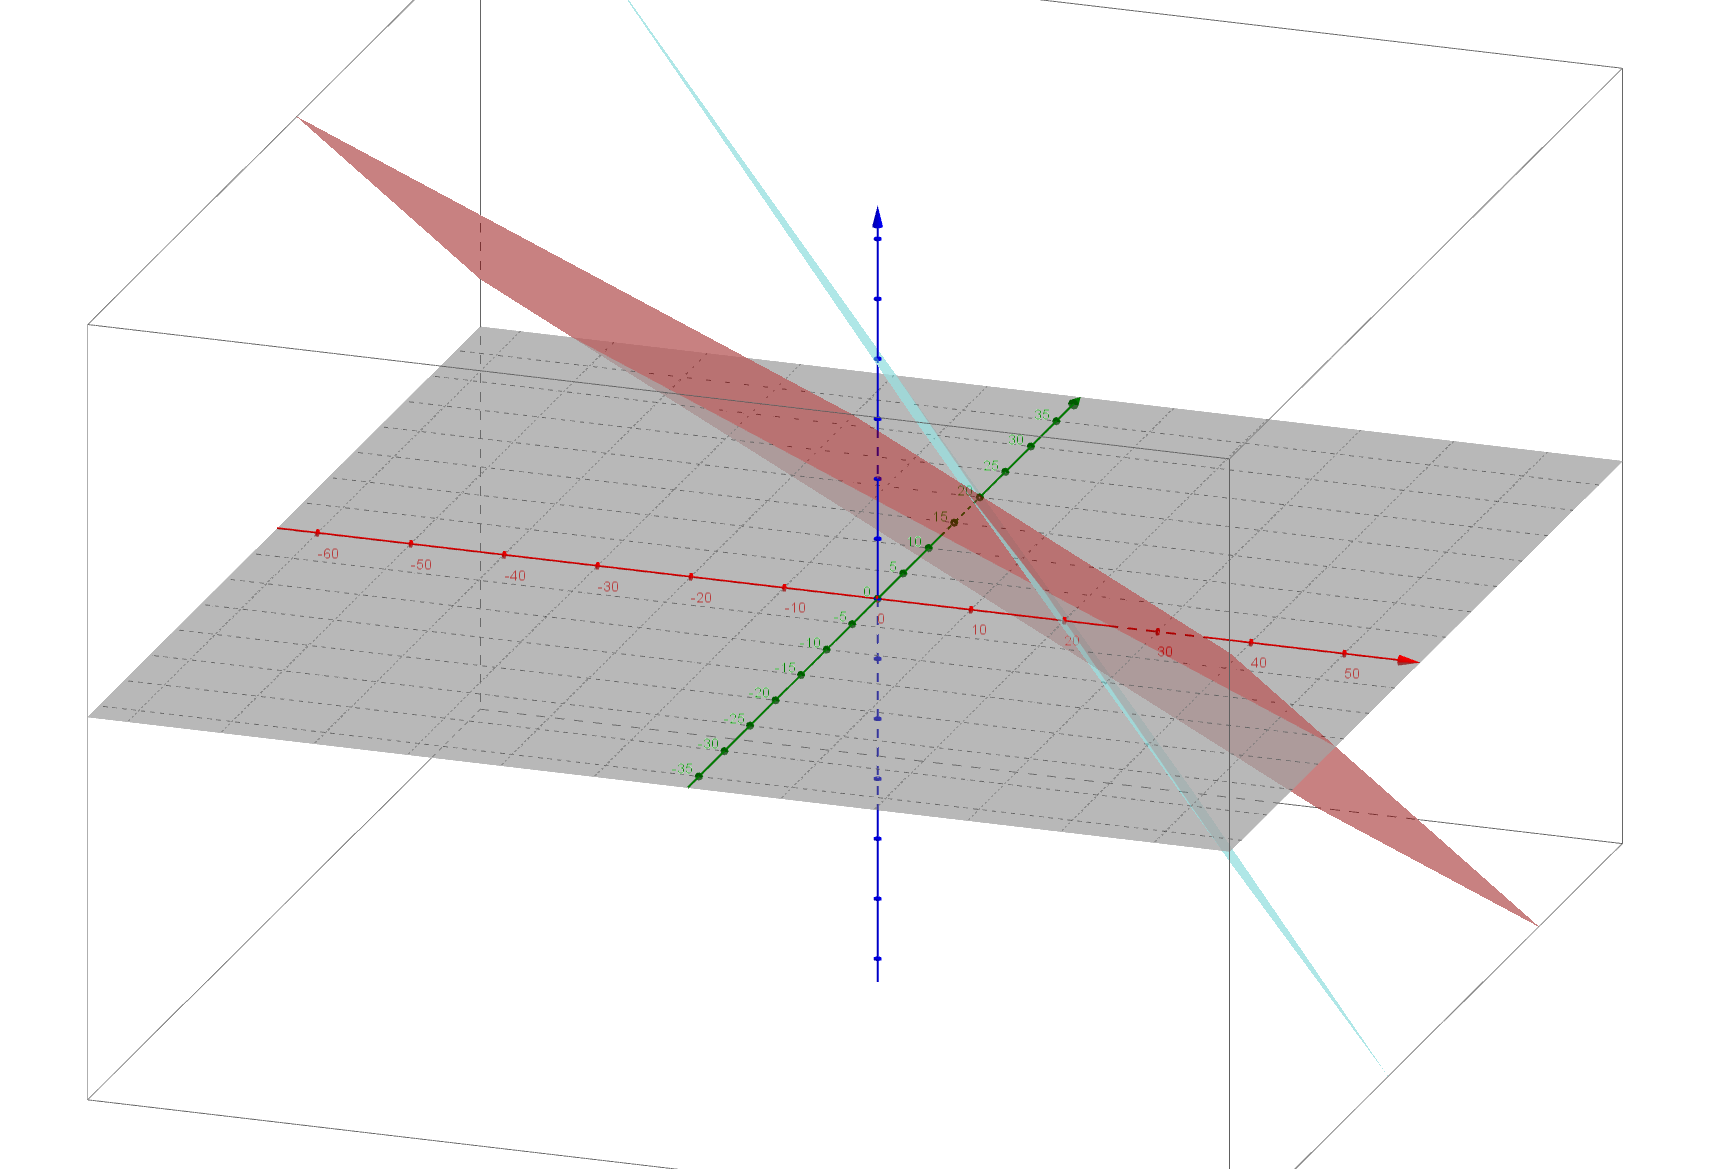
\includegraphics[width=340pt,height=270pt]{figure1.png}
    \caption{约束条件}
\end{figure}
\par \noindent \large \textcolor{blue}{给出matlab调用函数intLinprog函数的解法的模型化:}
    \par Matlab给出了求解线性规划的matlab标准型:\textbf{目标函数最小值、约束条件小于等于号或者等号。}\\倘若求最大值或约束条件有大于等于,可以添加-号使不等式变号。
    \\ 整数规划代码: $\left[  x,fval  \right]$ = intlinprog($f$,itcon,$A$,$b$,$Aeq$,$beq$,$lb$,$ub$,$x_0$)
    \par 其中,$f,x,b,beq,lb$和 $ub$ 是向量,$A$ 和$ Aeq$ 是矩阵。更加详细一点:
    \\$f$为目标函数的系数列向量
    \\intcon是标明哪些变量是整数变量
    \\ $A,b$为不等式约束条件的变量系数矩阵和常数项矩阵
    \\$Aeq,beq$为等式约束条件的稀疏矩阵和常数项矩阵
    \\$lb,ub$为决策变量的最小取值和最大取值
    \\$x_0$表示初始可行点,从这里开始优化
    \subsection{0-1规划matlab标准型}
    对于 0-1 规划问题,MATLAB 提供命令 bintprog 求解。 MATLAB 中 0-1 规划的标准形
式为:
\\$\min f'*X$
\par \noindent s.t.$\left\{\begin{matrix}
    A*X <= b,\\
Aeq*X = beq,
\end{matrix} \right.$
\\其中 X 的每个分量为 0 或者 1。
\\(1)X = BINTPROG(f) 求解问题 $\min f'*X$
\\(2)X = BINTPROG(f,A,b) 求解 $\min f'*X s.t. A*X <= b$
\\(3)X = BINTPROG(f,A,b,Aeq,beq)求解 $\min f'*X s.t. Aeq*X = beq, A*X <= b$
\section{线性规划-适用题目}

\subsection{线性规划适用的赛题:} 
在规划题目中,有些最优解可能是分数或小数,但是对于某些问题,有些或全部变量必须是整数,比如机器的台数,工作的人数或者装配的货物等等。这个时候就需要整数规划。
\\\textcolor{blue}{这个情况下无特定算法,只能近似模拟。}matlab只能求解0-1规划,对于其他整数规划也只能求出近似解,且没有相应的对应函数。
\begin{itemize}
    \item[·\textcolor{blue}{背包问题}] 设有一个背包,其最大承重为$ b$ ,考虑 $n $件物品,其中第 $j$ 件重量为 $a_j$ ,其价值为 $c_j$ 。问如何选取物品装入背包中,使得背包内物品的总价值最大?
    \item[·\textcolor{blue}{广义指派问题}] 设有 $m$ 台机器, $n$ 个工件,第 $i$ 台机器的可用工时数为 $b_i$ ,第 $i$ 台机器完成第 $j$ 件工件需要的工时数为 $a_{ij} $,费用为$ c_{ij} $。问如何最优指派机器生产。
    \item[·\textcolor{blue}{集合覆盖}] 设某地区划分为若干个区域,需要建立若干个应急服务中心(如消防站,急救中心等),每个中心的建立都需要一笔建站费用,设候选中心的位置已知,每个中心可以服务的区域预先知道,问如何选取中心使得应急服务能覆盖整个地区且使得建站费用最小。
\end{itemize}
\subsection{手写模型:}
1.~分枝定界法:不考虑整数类型变量,先对该松弛问题求解:
\\若该松弛问题无解,那么ILP问题一定无解。
\\若该松弛问题最优解符合整数条件,那么这个解一定是ILP问题最优解。
\\若不满足整数条件,那么可以任选一个不是整数的变量$x_i^0$来作为起始优化点,构造新的约束条件,$x_i \leq \left[x_i^0\right];x_i\geq \left[x_i^0\right]+1 $ ,添加到该松弛问题中形成两个子问题( $x_i$向下取整or向上取整作为上下界,添加约束)
\\依次在缩小的可行域中求解新构造的线性规划的最优解,并重复上述过程,直到子问题无解或有整数最优解。
\begin{figure}[H]
    \centering
    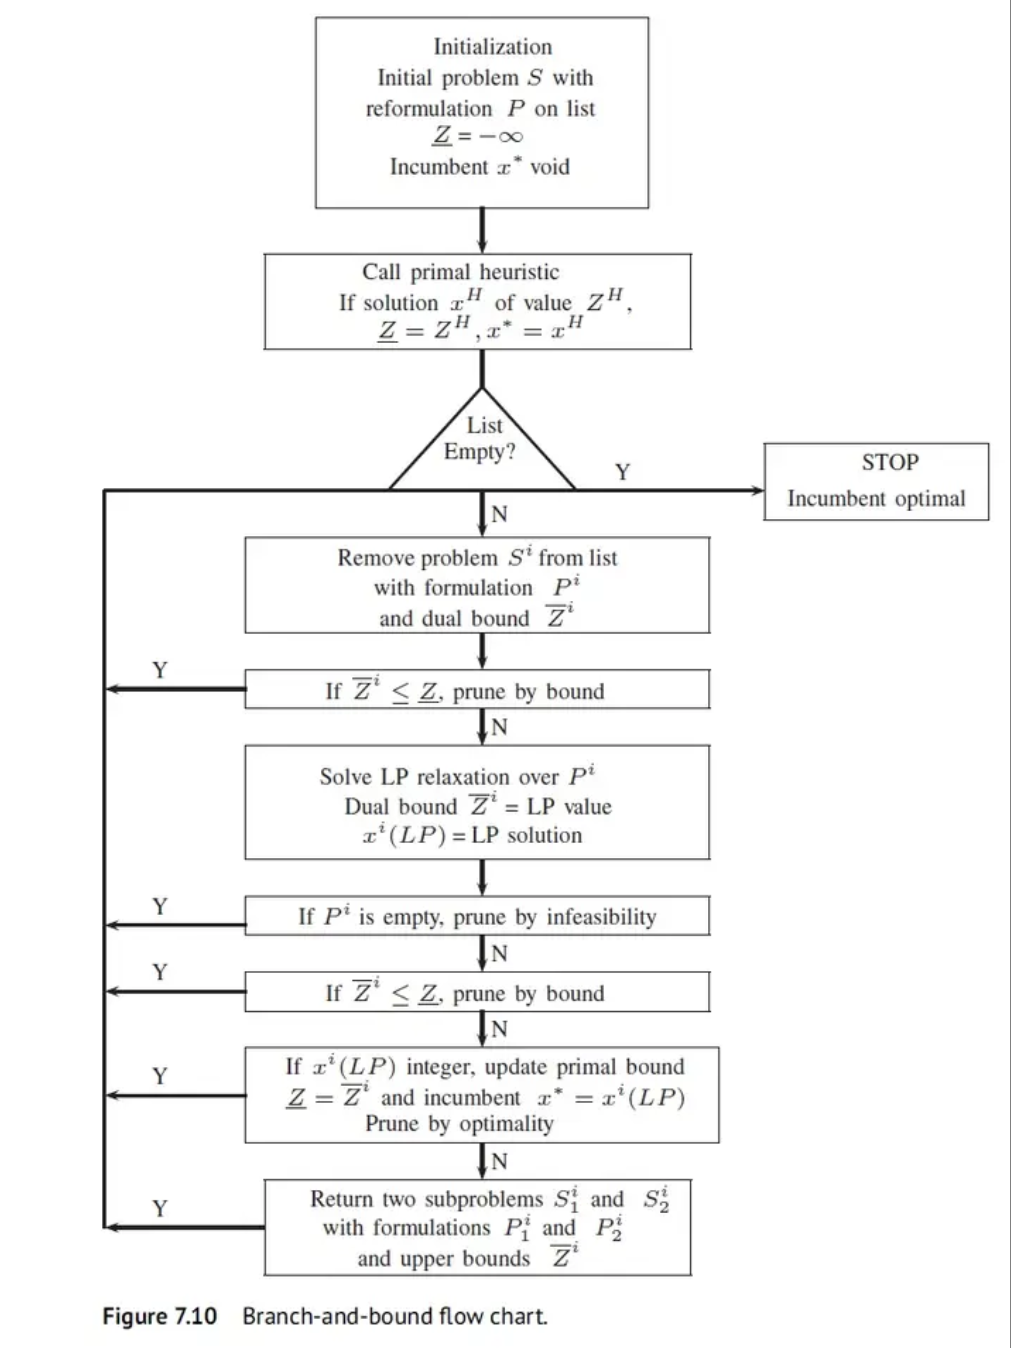
\includegraphics[width=340pt,height=270pt]{figure3.png}
    \caption{分支定界法图解}
\end{figure}
这个就是分支定界法的大概操作算法流程。从图中可以看到 初始化阶段 我们需要给定输出的 全局的上界 $\bar{z}$ 和下界 $\underline{z}$ ,如果能有一些启发式的方法获得稍微好点的上下界作为初始解导入那是最好的不过的了。如果没有的话可以先设置为正负无穷大。

接着进入到主循环中,我们通过求解整数规划的连续松弛问题(线性规划)来得到该子问题的上界。在主循环中,剩余的操作其实就是依据我们上一节所讲的四种情况来分别进行,即 Pruned by optimality,Pruned by bound,No pruning possible, Pruned by infeasibility,对于情况1,2,4我们需要提前跳出循环完成剪枝的过程。如果情况1,2,4都不满足的话,就会一直运行到最后一步 return two subproblems 因为没有剪枝,所以需要把两个子节点都添加进来。
\\2.~割平面法:同上,
\par \noindent(1)如果松弛问题(P0)无解,则(P)无解;

\par \noindent(2)如果(P0)的最优解为整数向量,则也是(P)的最优解;

\par \noindent(3)如果(P0)的解含有非整数分量,则对(P0) 增加割平面条件:即对(P0)增加一个线性约束,将(P0)的可行区域割掉一块,使得非整数解恰好在割掉的一块中, 但又没有割掉原问题(P)的可行解,得到问题(P1),重复上述的过程。
\begin{figure}[H]
    \centering
    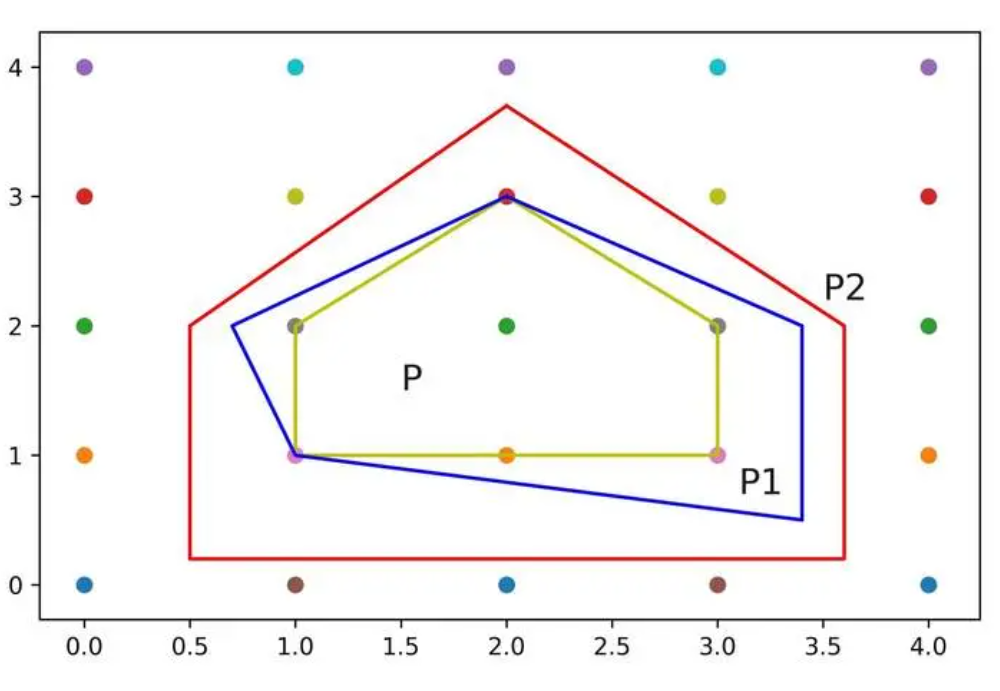
\includegraphics[width=340pt,height=270pt]{figure2.png}
    \caption{割平面法图解}
\end{figure}
\par \noindent 3.~匈牙利算法:大概就是计算指派问题最优解,这个其实可以看算法大全第二章,分别是先划去元素0,圈出独立元素0,打对勾,然后就给出了最优指派的解。
\\4.~过滤隐枚举法:简单来说,就是穷举,但是要根据约束条件判断符合条件来减少运算量。
\section{整数规划-代码实现}
\par 贴出matlab代码求解,请结合前面的式子来分别对应整数变量
    \begin{center}
    \begin{lstlisting}[caption={INP},language=Matlab]
        % IntLinear Programming(ILP)
        clc;clear;
        f=[-20,-30,-40];
        a=[4,8,10;1,1,1];
        b=[100;20];
        itcon=[1:1:3];
        [x,fval]=intlinprog(f,itcon,a,b,[],[],zeros(3,1));
        [x1,fval1]=linprog(f,a,b,[],[],zeros(3,1));
        disp('linprog(LP):')
        disp(x1)
        disp(fval1)
        disp('intlinprog(ILP):')
        disp(x)
        disp(fval)
        \end{lstlisting}
    \end{center}
    \section{整数规划-实战演练}
    国赛的难度基本上都可以说成是国家自然科学基金子课题全国征求意见稿了,你还搁这指整数规划能解决呢。欸,别急,还真可以,大多数国赛题都会有0-1规划,但是这玩意没有固定的算法,所以还是自己去找国赛题去看吧。
    \\记得去看我发的算法大全第二章,这波保底进度到这,里面题我做完发出来答案(虽然不保证正确),
    这章只将整数规划,结束,收工。



    \newpage
\begin{thebibliography}{99}  

    \bibitem{ref1}谢中华. MATLAB与数学建模[A].北京航空航天大学出版社[M]:科学技术协会,2021-02-14.
    \bibitem{ref2}21尔伊. 【数学建模学习】整数规划(MATLAB)[M]:2021-07-13.
    \bibitem{ref3}mathworks. 非线性规划问题求解器[J]:\url{https://ww2.mathworks.cn/help/optim/ug/linprog.html#description}
    % \bibitem{ref2}陈香敏,魏伟,吴莹. “文化+人工智能”视阈下文化创意产业融合发展实践及路径研究[A]. 中共沈阳市委、沈阳市人民政府.第十七届沈阳科学学术年会论文集[C].中共沈阳市委、沈阳市人民政府:沈阳市科学技术协会,2020:4.
    % \bibitem{ref3}田晓曦,刘振鹏,彭宝权. 地方高校开展教育人工智能深度融合的路径探究[A]. 中共沈阳市委、沈阳市人民政府.第十七届沈阳科学学术年会论文集[C].中共沈阳市委、沈阳市人民政府:沈阳市科学技术协会,2020:5.
    % \bibitem{ref4}柏卓君,潘勇,李仲余.彩色多普勒超声在早期胚胎停育诊断中的应用[J].影像研究与医学应用,2020,4(18):129-131.
    % \bibitem{ref5}杨芸.我院2018年人血白蛋白临床应用调查与分析[J].上海医药,2020,41(17):34-35+74.
    
    \end{thebibliography}

    \newpage
    \section{数学建模算法大全第二章习题答案}
\begin{itemize}
    \item[1]首先假设决策变量:四个班次的人数分别为$x_i(i=1,\cdots,4)$
    \\那么可以得出:\begin{table}[H]
        \begin{tabular}{|c|c|c|c|}
            \hline
            时间 & 8-12 & 10-12 & 12-14 \\ 
            \hline
            人数 & $x_1+x_2$ & $x_1+x_2$ &$x_1+x_3+x_4,x_2+x_3+x_4$ \\
            \hline
            14-16 &  &16-18 &18-21\\
            \hline
            $x_1+x_2+x_3+x_4$ & & $x_1+x_2+x_4,x_3$ & $x_3+x_4$ \\
            \hline
        \end{tabular}
    \end{table}
    \par \noindent  
    
        目标函数 $\min y = 800x_1 + 800x_2+900x_3+900x_4$
        \\同时给出约束条件
        \\s.t.$\left\{\begin{matrix}
            x_1+x_2 \geqslant  20\\
            x_1+x_2 \geqslant  25\\
            x_1+x_3+x_4 \geqslant  10\\
            x_2+x_3+x_4 \geqslant  10\\
            x_1+x_2+x_3+x_4 \geqslant  30\\
            x_3 \geqslant 20\\
            x_1+x_2+x_4 \geqslant  20\\
            x_3+x_4 \geqslant  10\\
        \end{matrix}\right.$
        
    \par \noindent 然后就可以给出结果$ x_1=0
    ,x_2=25
    ,x_3=20
    ,x_4=0,\min Z=38000$
\end{itemize}
\end{document}